
% Digital Logic Report Template
% Created: 2020-01-10, John Miller

%==========================================================
%=========== Document Setup  ==============================

% Formatting defined by class file
\documentclass[11pt]{article}

% ---- Document formatting ----
\usepackage[margin=1in]{geometry}	% Narrower margins
\usepackage{booktabs}				% Nice formatting of tables
\usepackage{graphicx}				% Ability to include graphics

%\setlength\parindent{0pt}	% Do not indent first line of paragraphs 
\usepackage[parfill]{parskip}		% Line space b/w paragraphs
%	parfill option prevents last line of pgrph from being fully justified

% Parskip package adds too much space around titles, fix with this
\RequirePackage{titlesec}
\titlespacing\section{0pt}{8pt plus 4pt minus 2pt}{3pt plus 2pt minus 2pt}
\titlespacing\subsection{0pt}{4pt plus 4pt minus 2pt}{-2pt plus 2pt minus 2pt}
\titlespacing\subsubsection{0pt}{2pt plus 4pt minus 2pt}{-6pt plus 2pt minus 2pt}

% ---- Hyperlinks ----
\usepackage[colorlinks=true,urlcolor=blue]{hyperref}	% For URL's. Automatically links internal references.

% ---- Code listings ----
\usepackage{listings} 					% Nice code layout and inclusion
\usepackage[usenames,dvipsnames]{xcolor}	% Colors (needs to be defined before using colors)

% Define custom colors for listings
\definecolor{listinggray}{gray}{0.98}		% Listings background color
\definecolor{rulegray}{gray}{0.7}			% Listings rule/frame color

% Style for Verilog
\lstdefinestyle{Verilog}{
	language=Verilog,					% Verilog
	backgroundcolor=\color{listinggray},	% light gray background
	rulecolor=\color{blue}, 			% blue frame lines
	frame=tb,							% lines above & below
	linewidth=\columnwidth, 			% set line width
	basicstyle=\small\ttfamily,	% basic font style that is used for the code	
	breaklines=true, 					% allow breaking across columns/pages
	tabsize=3,							% set tab size
	commentstyle=\color{gray},	% comments in italic 
	stringstyle=\upshape,				% strings are printed in normal font
	showspaces=false,					% don't underscore spaces
}

% How to use: \Verilog[listing_options]{file}
\newcommand{\Verilog}[2][]{%
	\lstinputlisting[style=Verilog,#1]{#2}
}




%======================================================
%=========== Body  ====================================
\begin{document}
	
	\title{ELC 2137 Lab 02: Transistor Logic Gates}
	\author{Yiting Wang}
	
	\maketitle
	
	
	\section*{Summary}
	
		Gates are made up of switches (on/off). How you connect them determines the type of gate; Transistors are “voltage-controlled switches,” so we can hook gates together.  \\
		
	
	
	\section*{Q\&A}
	
	\begin{enumerate}
		\item What logic operation does it implement?\\
		it's AND gate\\
	\end{enumerate}
	
	
	
	\section*{Results}
	
		Table 1 is the truth table for the final gate I did in the lab. I keeped my NOR gate, and built two more inverters, then I connected one to each input (between the switch and the transistor of the NOR gate).   The truth table shows that the final gate is an AND gate.\\
	\begin{table}[ht]\centering
		\caption{Logic/truth table for the Final gate}
		\label{tbl:example_table}
		\begin{tabular}{cc|c}
			\toprule
			A & B & LED \\
			\midrule
			0 & 0 & 0 \\
			0 & 1 & 0 \\
			1 & 0 & 0 \\
			1 & 1 & 1 \\
			\bottomrule
		\end{tabular}
	\end{table}
	
		Figure 1 and 2 are the circuit demonstration page I completed, they include the instuctor initials and the current paths for inverter, NOR gate, and final gate.\\
	\begin{figure}[ht]\centering
		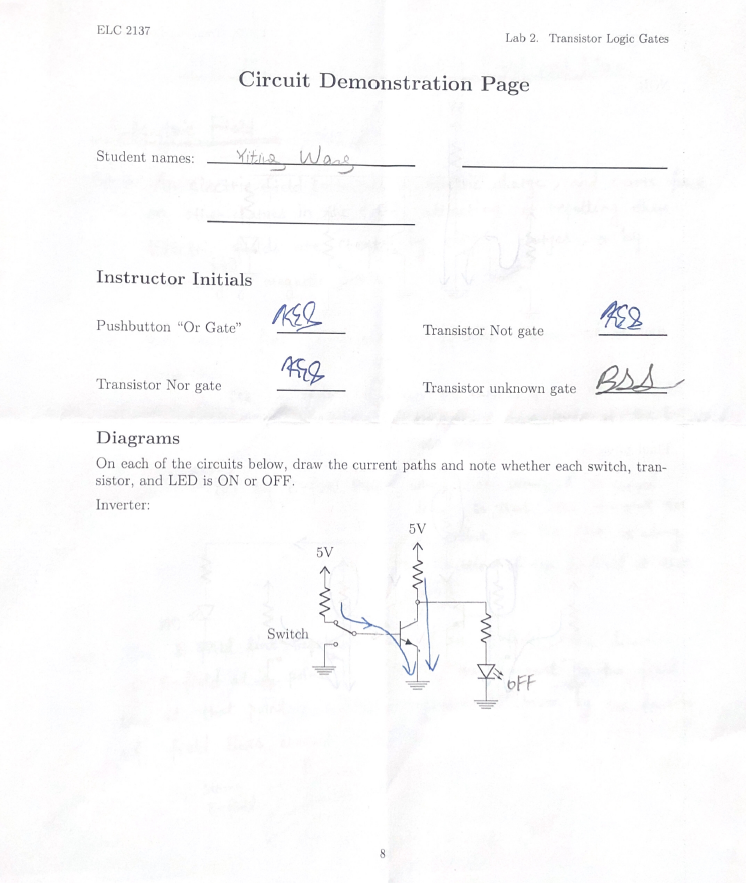
\includegraphics[width=1.0\textwidth]{Lab2Page1}
		\caption{This is the Circuit Demonstration Page 1.}
		\label{fig:original_logo}
	\end{figure}
	
	\begin{figure}[ht]\centering
		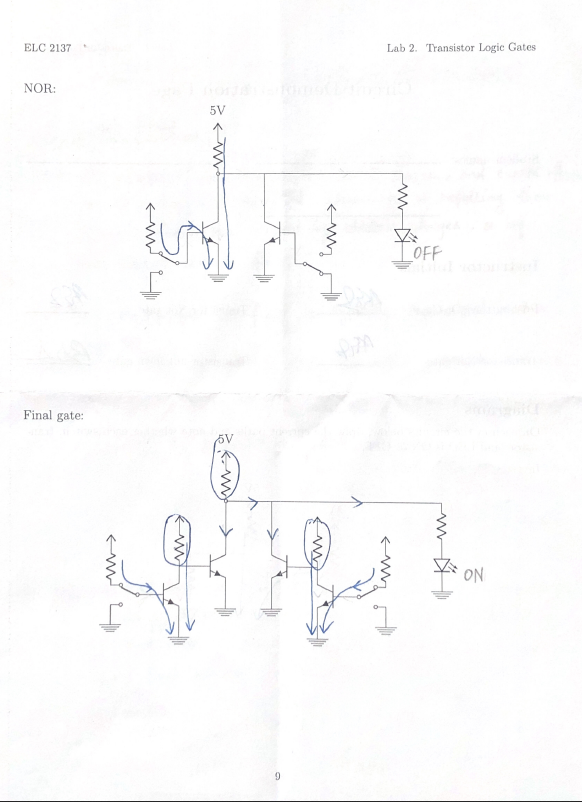
\includegraphics[width=1.0\textwidth]{Lab2Page2}
		\caption{This is the Circuit Demonstration Page 2.}
		\label{fig:original_logo}
	\end{figure}
	
	
	
	\section*{Code}
	
	There is no code require in this lab.\\
	
	
	
\end{document}
